最後に$\varphi$が全単射であることを証明する.そのために次の概念を導入する.

\begin{defin}
  path $p_1,\cdots,p_k$を$1$辺の長さが$n+k$の正三角形に図\ref{generic puzzle}のように配置したとき,重なってしまうpieceが存在する場合,このpuzzle $P$はskew puzzleであると呼ぶ.
\end{defin}

skew puzzleに対しても$\varphi$によってedge labeled tableauxを対応させることができるが,次の補題が成り立つ.

\begin{lemm}\label{skew puzzle}
  $P$がskew puzzleであることと$\text{EqRect}(\varphi(P))\neq T_{\mu}$であることは同値である.
\end{lemm}

\begin{proof}
  命題\ref{main theorem 1}より,$\text{EqRect}(\varphi(P))\neq T_{\mu}$ならば$P$はskewではない.

  
\end{proof}

\begin{prop}
  $\varphi\colon\mathcal{P}^\nu_{\lambda\mu}\rightarrow\mathcal{T}^\nu_{\lambda\mu}$は全単射である.
\end{prop}

\begin{proof}
  $T\in \mathcal{T}^\nu_{\lambda\mu}$に対して,path $p_1,\cdots,p_k$をつぎのように定める.

  まず$p_k$のsegment $s_{k,1}$を決定する.piece 
  
\begin{tikzpicture}[baseline=-1pt]
    \fill[cyan] (0,0)--(0.25,0.42)--(0.5,0)--(0.25,-0.42)--cycle;
    \draw[thick] (0,0)--(0.25,0.42)--(0.5,0)--(0.25,-0.42)--cycle;
  \end{tikzpicture}
  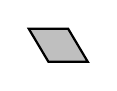
\begin{tikzpicture}[baseline=2pt]
    \fill[lightgray] (0,0)-- ++(0.5,0)-- ++(-0.25,0.42)-- ++(-0.5,0)--cycle;
    \draw[thick](0,0)-- ++(0.5,0)-- ++(-0.25,0.42)-- ++(-0.5,0)--cycle;
  \end{tikzpicture}
  
\begin{tikzpicture}[baseline=2pt]
    \fill[yellow] (0,0)-- ++(0.5,0)-- ++(0.25,0.42)-- ++(-0.5,0)--cycle;
    \draw[thick](0,0)-- ++(0.5,0)-- ++(0.25,0.42)-- ++(-0.5,0)--cycle;
  \end{tikzpicture}
  それぞれ文字 $text{b},\text{g},\text{y}$と同一視し,segment に含まれるpiece を上から読んで,$text{b},\text{g},\text{y}$からなる文字列と同一視する.

  $T$の$k$行目の最も右にある箱を$x$とおく.$\alpha = |\mu|$,$s_{k,1}$は空の文字列とする.
  \[
  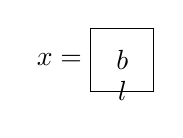
\begin{tikzpicture}
    \node at (-0.4, -0.4) {$x=$};
    \draw (0,0) rectangle ++(0.8,-0.8);
    \node at (0.4,-0.4) {$b$};
    \node at (0.4,-0.8) {$l$};
  \end{tikzpicture}
  \]
  としたとき,$\alpha = b$ならば$s_{k,1}$の左に$\text{y}$を付け足す.$\alpha\in l$ならば$s_{k,1}$の左に$\text{b}$を付け足す.$\alpha\neq b$かつ$\alpha\notin l$ならば$s_{k,1}$の左に$\text{g}$を付け足す.$x$の左に箱が存在するならば$x$を$x$の左の箱に置き換え,$\alpha$を$\alpha -1$に置き換えて同じ操作をする.$x$の左に箱が存在しないならば操作を終了する.

  次に$s_{k-1,2}$を決定する.$\alpha$は$s_{k,1}$に対する操作が終了したときと同じまま,$x$は$T$の$k-1$行目の最も右にある箱とする.


  
  補題\ref{skew puzzle}より$p_1,\cdots,p_k$はpuzzle $P$を定め,$\varphi(P)=T$である.

  $\varphi(P)=\varphi(P')$であるならば,$P$と$P'$に含まれるpathは等しいから,$P=P'$でなければならない.
\end{proof}



% k=1の場合はwt(T)\neq 0であるということから\varphi(P) = Tなる$P$が存在することがわかる.

$k$に関する帰納法で示す.$k=1$として,$\lambda=(l)$,$\mu=(m)$,$\nu=(n)$とする.$\text{EqRect}(T)=T_{(m)}$と$\text{wt}(T)\neq 0$より,次が成り立つ.
  \begin{enumerate}
    \item box labelの入った箱はedge labelを持たない.
    \item $T$のすべてのedge labelはたかだか$1$つの要素しか持たない.
    \item ある$r\in\integer$が存在して$1,\cdots,r$はすべて$T$のedge labelに現れ,$r+1,\cdots,m$はすべて$T$のbox labelに現れる.
    \item $T$のlabelを左から順に読んでいくとちょうど$1,2,\cdots,m$の順で並ぶ.
  \end{enumerate}
  
  したがって$T$は図\ref{1 row tableaux}のような形になる.
  \begin{figure}[h]
    \centering
    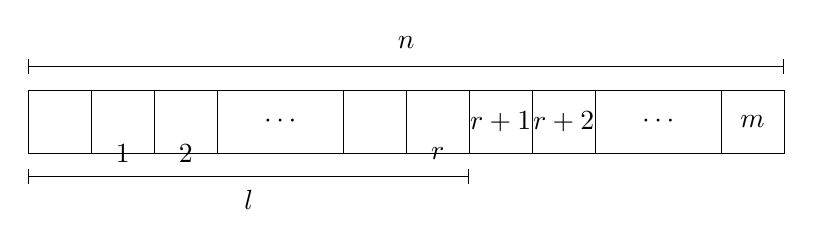
\begin{tikzpicture}
      \draw (0,0) rectangle ++(12 * 0.8, 0.8);
      \foreach \x in {1,2,3,5,6,7,8,9,11} {
        \draw (\x * 0.8, 0) -- (\x * 0.8, 0.8);
      } 

      \draw[|-|] (0, -0.3) -- ++(7 * 0.8, 0);
      \node at (2.8, -0.6) {$l$};

      \draw[|-|] (0, 1.1) -- ++(12 * 0.8, 0);
      \node at (4.8, 1.4) {$n$};

      \node at (1.2, 0) {$1$};
      \node at (2, 0) {$2$};
      \node at (5.2, 0) {$r$};
      \node at (3.2, 0.4) {$\cdots$};
      \node at (6,0.4) {$r+1$};
      \node at (6.8,0.4) {$r+2$};
      \node at (8,0.4) {$\cdots$};
      \node at (9.2,0.4) {$m$};
    \end{tikzpicture}
    \caption{}\label{1 row tableaux}
  \end{figure}
  よって$\psi(T)=p_1$はpuzzleを定め,$\varphi(\psi(T))=T$である.
